\documentclass[a4paper,12pt]{article}
\usepackage{geometry}
\usepackage{fullpage} % Package to use full page
\usepackage{parskip} % Package to tweak paragraph skipping
\usepackage{amsmath}
\usepackage{hyperref}
\usepackage{amsmath,amsfonts,amsthm} % Math packages
\usepackage{graphicx}
\usepackage{listings}
\usepackage{color}
\usepackage{float}
\definecolor{codegreen}{rgb}{0,0.6,0}
\definecolor{codegray}{rgb}{0.5,0.5,0.5}
\definecolor{codepurple}{rgb}{0.58,0,0.82}
\definecolor{backcolour}{rgb}{0.95,0.95,0.92}
\definecolor{brown}{rgb}{0.59, 0.29, 0.0}
\definecolor{beaublue}{rgb}{0.74, 0.83, 0.9}
\definecolor{orange}{rgb}{1.0, 0.5, 0.0}
\definecolor{darkslategray}{rgb}{0.18, 0.31, 0.31}
\def\Xint#1{\mathchoice
	{\XXint\displaystyle\textstyle{#1}}%
	{\XXint\textstyle\scriptstyle{#1}}%
	{\XXint\scriptstyle\scriptscriptstyle{#1}}%
	{\XXint\scriptscriptstyle\scriptscriptstyle{#1}}%
	\!\int}
\def\XXint#1#2#3{{\setbox0=\hbox{$#1{#2#3}{\int}$}
		\vcenter{\hbox{$#2#3$}}\kern-.5\wd0}}
\def\dashint{\Xint-}

% Swap the definition of \abs* and \norm*, so that \abs
% and \norm resizes the size of the brackets, and the 
% starred version does not.
\makeatletter
\let\oldabs\abs
\def\abs{\@ifstar{\oldabs}{\oldabs*}}
%
\let\oldnorm\norm
\def\norm{\@ifstar{\oldnorm}{\oldnorm*}}
\makeatother
\lstdefinestyle{mystyle}{
	backgroundcolor=\color{white},   
	commentstyle=\color{codegreen},
	keywordstyle=\color{blue},
	identifierstyle=\color{brown},
	numberstyle=\tiny\color{codegray},
	stringstyle=\color{orange},
	basicstyle=\footnotesize,
	breakatwhitespace=false,         
	breaklines=true,                 
	captionpos=b,                    
	keepspaces=true,                 
	numbers=left,                    
	numbersep=5pt,                  
	showspaces=false,                
	showstringspaces=false,
	showtabs=false,                  
	tabsize=2
}
\lstset{style=mystyle}

\title{\normalsize AMATH 535: Homework Problem 3.7 (Extra Credit)}
\author{\normalsize Jithin D. George, No. 1622555}
% matrix environment
\newenvironment{mat}{\left[ \begin{array}{ccccccccccccc}}{\end{array}\right]}
\newcommand\bcm{\begin{mat}}
	\newcommand\ecm{\end{mat}}

\begin{document}

\maketitle
	
{\bf A Statistician’s Revenge (Extra Credit)	} 


Fifty ungulates (hoofed, grazing mammals) are introduced to a
uninhabited island. These ungulates have the following characteristics:

$\beta$ = 0. 15 ungulates per individual per year ,

$\mu$ = 0. 05 ungulates per individual per year .

How long should you wait to revisit the island to be 95 \% sure that the
population has doubled ?

Hint: Think of each of the 50 introduced ungulates as a separate birth
and death process. Feel free to use the central limit theorem.

{\bf Solution:	}


I listen to the wise hint and think each of the 50 as separate birth and death process. So, the initial population is 1 and we have 50 such populations.

For such a process, the P.G.F is given by
\[ F = \frac{0.05(1-x)e^{rt} + 0.15x-0.05}{0.15(1-x)e^{rt} + 0.15x-0.05} =  \frac{(1-x)e^{rt} + 3x-1}{3(1-x)e^{rt} + 3x-1} \]

\[r = \beta - \mu = 0.1 \]
So,
\[ F =  \frac{(1-x)e^{0.1t} + 3x-1}{3(1-x)e^{0.1t} + 3x-1} \]

The mean and the variance are given by
\[E = n_0 e^{0.1t}= e^{0.1t} \]
\[Var = 2e^{0.1t}(e^{0.1t}- 1) \]
Thus, the standard deviation is 
\[ \sigma = \sqrt{2e^{0.1t}(e^{0.1t}- 1)}\]

According to the Central Limit theorem, given a large enough sample size, the distribution of the samples approaches a normal distribution. We believe 50 is a large enough sample size.

So, for us to be 95\% sure that the population at at least doubles, the probability that the population is extinct or the same must be two standard deviations away from the mean.
\[p_0(t) +p_1(t) < E(t) - 2\sigma \]
\[p_0 = F(0,t) = \frac{e^{0.1t} -1}{3e^{0.1t} -1}\]
\[p_1 = F_x(0,t) = \frac{(-e^{0.1t} + 3)(3(1-x)e^{0.1t} + 3x-1) -(-3e^{0.1t} + 3)((1-x)e^{0.1t} + 3x-1)}{(3(1-x)e^{0.1t} + 3x-1)^2} \big|_{x=0} \]
\[ =  \frac{(-e^{0.1t} + 3)(3e^{0.1t} -1) -(-3e^{0.1t} + 3)(e^{0.1t}  -1)}{(3e^{0.1t} -1)^2}\]
\[ =  \frac{4e^{0.1t}}{(3e^{0.1t} -1)^2}\]

Thus, we have 

\[\frac{e^{0.1t} -1}{3e^{0.1t} -1} +\frac{4e^{0.1t}}{(3e^{0.1t} -1)^2}<e^{0.1t} -2\sqrt{2e^{0.1t}(e^{0.1t}- 1)}\]

This looks so nasty. Let's try replacing $e^{0.1t}$ by x.

\[\frac{x -1}{3x -1} +\frac{4x}{(3x -1)^2}<x -2\sqrt{2x(x- 1)}\]

Still, nasty and not simply solvable by hand. Feeding this into Wolfram yields that there are no real solutions.

Thus, we get a seemingly wrong (?) result of no time when there is a 95 \% probability of seeing the population double. Although the birth rate is thrice the death rate, this result stems from the variance growing exponentially with time.

The dubious nature of this results demands some verification. After all, if we march for science, we must leave no stone unturned in our path. So, we use a computer in a different way : graphical results. 
Let's construct the function g such that
\[g(t)= E- 2\sigma-p_0 - p_1 \]
We want to find where g $>$ 0.
\begin{figure}[H] 
	\centering
	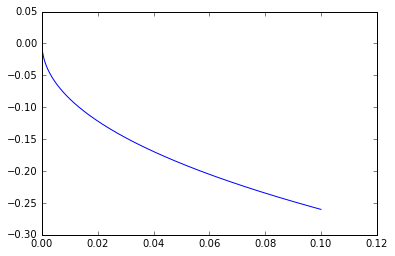
\includegraphics[width=14cm]{37a}
	\caption{g(t)over t}
	\end{figure}

This shows that Wolfram's result is not inaccurate.  If we plot the function without the standard deviations, we get the following plot.
\begin{figure}[H] 
	\centering
	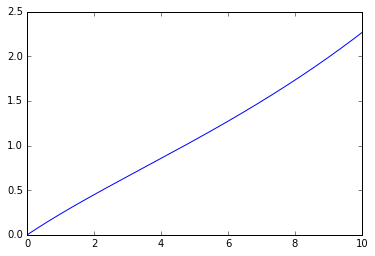
\includegraphics[width=12cm]{37b}
	\caption{$E-p_0 - p_1$over t}
\end{figure}

So, it seems that the standard deviation is the culprit that grows exponentially and make us  unable of being 95\% sure.

\end{document}